\documentclass[a4paper,10pt,twocolumn]{article}

\usepackage[utf8x]{inputenc}
\usepackage[french]{babel}
\usepackage{graphicx,times}
\usepackage[T1]{fontenc}
\usepackage{amsmath,amssymb}
\usepackage[font=footnotesize]{caption}
\usepackage{fancyhdr}
\usepackage[explicit]{titlesec}
\usepackage{hyperref}
%\usepackage[square,comma,numbers]{natbib}
\usepackage{tabularx}
\usepackage{xcolor}

%for columns spanning multiple rows in tables
\usepackage{multirow}
%use the booktabs package to get (much!) better vertical spacing above and below "rules" (horizontal lines), resulting in a much more professional look of your tables.
%use the colortbl package to add color to tables.
\usepackage{booktabs,colortbl}

% Petits extras:
\usepackage{textcomp} % Symbole Euro € \texteuro

\providecommand{\abs}[1]{\lvert#1\rvert}
\providecommand{\norm}[1]{\lVert#1\rVert}
\providecommand{\avg}[1]{\langle#1\rangle}

% détails, en gris: (e.g. std in table)
\providecommand{\deta}[1]{\textcolor{gray}{#1}}



\newcolumntype{L}[1]{>{\raggedright\arraybackslash}p{#1}}
\newcolumntype{C}[1]{>{\centering\arraybackslash}p{#1}}
\newcolumntype{R}[1]{>{\raggedleft\arraybackslash}p{#1}}

%\renewcommand{\bibsection}{}
%\def\bibfont{\footnotesize}
%\setlength{\bibsep}{0.2em}
%\setlength{\bibhang}{10em}

\hypersetup{colorlinks=true, urlcolor=blue, urlbordercolor={0 0 1}, citecolor=black, citebordercolor={1 1 1}}

\addto\captionsfrench{\def\figurename{Fig.}}
\addto\captionsfrench{\def\tablename{Tableau}}

\captionsetup[figure]{labelsep=period, justification=raggedright, singlelinecheck=false}
\captionsetup[table]{labelsep=period, justification=centering, singlelinecheck=false}

\parindent 10pt

\setlength{\voffset}{-1.3in}
\setlength{\topmargin}{1.25cm}
\setlength{\headheight}{1.125cm}
\setlength{\headsep}{0cm}

\setlength{\hoffset}{-1in}
\setlength{\oddsidemargin}{1.3cm}
\setlength{\evensidemargin}{1.3cm}

\setlength{\textheight}{25cm}%23.5
\setlength{\textwidth}{18.5cm}

\setlength{\headsep}{0.67cm}
\setlength{\columnwidth}{8.75cm}
\setlength{\columnsep}{0.63cm}

\setlength{\abovecaptionskip}{0em}
\setlength{\belowcaptionskip}{0em}

\titleformat{\section}
  {\normalfont}{\thesection.}{0.5em}{\MakeUppercase{#1}}
\titleformat{\subsection}
  {\normalfont\itshape}{\thesubsection.}{1.5em}{#1}
\titleformat{\subsubsection}
  {\normalfont\itshape}{\thesubsubsection.}{1.5em}{#1}
	
\titlespacing\section{0pt}{1em}{0.5em}
\titlespacing\subsection{0pt}{1em}{0.5em}
\titlespacing\subsubsection{0pt}{1em}{0.5em}

\fancyhf{}
\fancyhead[R]{\fontsize{8pt}{8pt}\selectfont \textbf{S}YMPOSIUM DE \textbf{G}ENIE \textbf{E}LECTRIQUE (SGE 2018), 3-5 JUILLET 2018, NANCY, FRANCE}
\renewcommand{\headrulewidth}{0pt}


\pagestyle{empty}


\title{
\fontsize{24pt}{24pt}\selectfont
Gestion d'énergie avec entrées incertaines : \\
quel algorithme choisir ?\\
Benchmark open source sur une maison solaire
}

\newcommand\tsp[1]{\textsuperscript{#1}}
\newcommand\sub[1]{\textsubscript{#1}}


\author{
\fontsize{11pt}{11pt}\selectfont
Pierre HAESSIG\tsp{*}, Jesse James PRINCE AGBODJAN\tsp{*}, Romain BOURDAIS\tsp{*}, Hervé GUÉGUEN\tsp{*}\\
\fontsize{10pt}{10pt}\selectfont
\tsp{*}IETR, CentraleSupélec
}

\date{}


\begin{document}

\maketitle
\thispagestyle{fancy}


\fontsize{9pt}{9pt}\selectfont
\textbf{RÉSUME --
Le pilotage optimal des systèmes énergétiques nécessite l'emploi d'algorithmes
de gestion optimale.
Ces outils se rattachent à théories de disciplines variées (Automatique, Optimisation, Recheche Opérationnelle),
qui ont chacune leur spécificité tout en se recouvrant partiellement.
%
Il est donc difficile, pour la personne ``non-initiée'', de saisir les principales caractéristiques
de chaque approche pour pouvoir les comparer et finalement trouver
quelles méthodes sont plus adaptées à un problème donné.
%
Pour permettre une comparaison objective et transparente,
nous proposons de problème simple de gestion d'énergie : une maison solaire 
avec production photovoltaïque et stockage, dont nous justifions le dimensionnement.
Ce benchmark accessible en ligne est open source et multi-langage (Python, Julia et Matlab).
Nous l'illustrons par une première comparaison de quelques méthodes de gestion d'énergie
(règle heuristique, MPC et optimisation anticipative)
et nous soulignons en particulier l'effet de l'incertitude
sur la production solaire.
% Extrait de l'ancien résumé, avec des idées à reprendre?
% comparer différentes méthodes en soulignant en particulier les investissements
% en temps à prévoir :
% temps pour la compréhension du cadre théorique,
% temps pour la modélisation du problème dans ce cadre,
% temps pour l'implémentation numérique et la validation des résultats.
}\\

\textbf{\textit{Gestion d'énergie, Optimisation dynamique, Optimisation stochastique,
Commande prédictive, Autoconsommation photovoltaïque}}

\fontsize{10pt}{10pt}\selectfont


\section{Introduction}

De très nombreux travaux de recherche portent sur le pilotage des systèmes énergétiques
pour optimiser leur fonctionnement.
Les méthodes de gestion d'énergie, développées depuis les années 1950,
sont nombreuses et variées (cf. partie \ref{s:opt_meth}).
Ainsi, la personne qui aborde un problème de gestion d'énergie
est confrontée à un choix qui est souvent difficile à \emph{objectiver}.
En effet, les difficutés associées à chaque méthode sont de nature divers:
difficultés de compréhension du cadre théorique, difficultés d'implémentation
numérique ou de temps de calcul, et parfois existence de
``dépendances cachées''\footnote{exemples de dépendance:
la méthode ``commande prédictive'' (MPC) nécessite d'avoir des prévisions des entrées incertaines.
Beaucoup d'autres méthodes nécessitent des modèles statistiques de ces entrées.}
Malheureusement, les méthodes a priori les plus performantes du point de vue de l'optimalité
cumulent la plupart des ces difficultés.
Dès lors, la personne face au choix pourrait avoir peur d'investir beaucoup de son temps
dans une méthode ``complexe'' si elle n'a pas une certaine assurance d'obtenir une meilleure
performance qu'avec une méthode ``simple''.

Pour sortir de ce dilemme, nous souhaitons faciliter la \emph{comparaison objective},
sans préjugés, des méthodes de gestion d'énergie.
Nous proposons donc un \emph{banc de test de gestion d'énergie open source}.
Il permet, sur un exemple simple, mais pertinent, d'avoir un aperçu de différentes méthodes
de pilotage\footnote{``pilotage'', ``gestion'', ``commande'', ``optimisation''...
le vocabulaire change selon les disciplines ou le contexte.
Nous utilisons ici ces termes de façon interchangeable.}.
Ce benchmark doit permettre de comparer les comparer
à la fois du point de vue de la performance (optimalité du résultat),
mais aussi de comparer leur mise en oeuvre, en particulier l'implémentation
dans différents langages de programmation.

Il existe des travaux comparant des méthodes de gestion d'énergie, sur des exemples réels complexes
(barrages hydroélectriques \cite{Zambelli:2011:SBA}, véhicules hybrides \cite{Jiang:2017:ToVT}).
Notre proposition est complémentaire, car elle porte au moins autant sur la comparaison \emph{fonctionnelle}
des méthodes (e.g. analyse des objets nécessaires pour leur mise en oeuvre) que
sur la comparaison quantitative des résultats d'optimisation.
Par ailleurs, notre proposition est librement accessible à tous (code et données open source).

\section{Banc de test: maison solaire}

\subsection{Modèle de la maison solaire}
\label{ss:model}

\begin{figure}[!ht]
        \begin{center}
                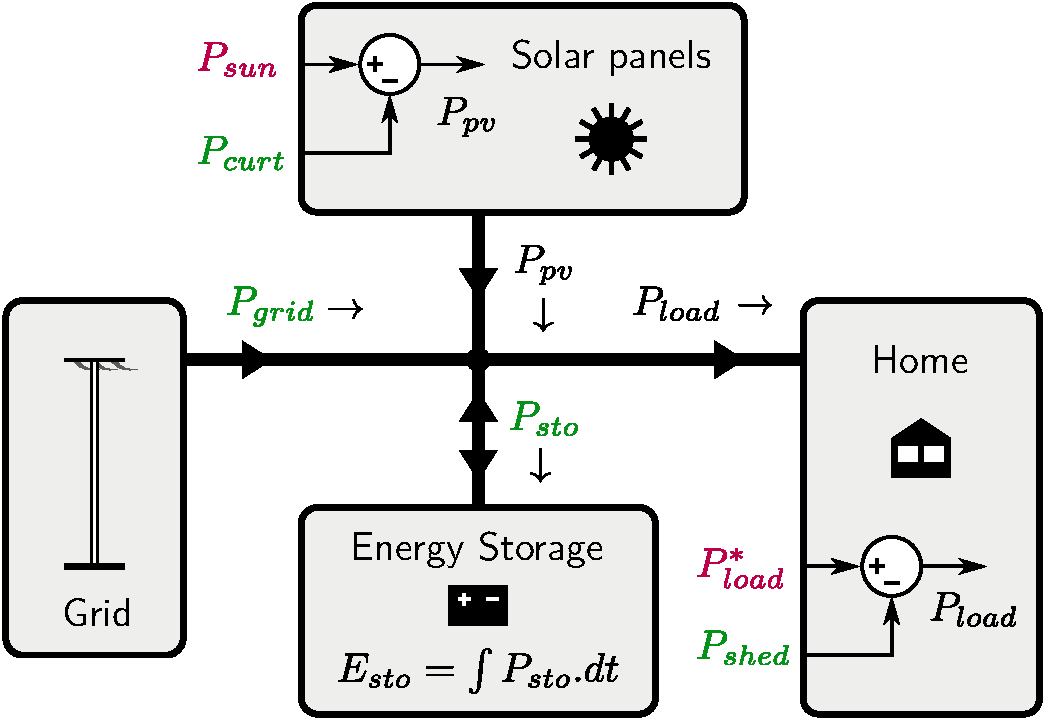
\includegraphics[width=0.9\columnwidth]{figures/solar_home.pdf}
        \end{center}

        \caption{Modèle en flux d'énergie de la maison solaire.
        Variables de décision en vert, données externes en rouge (potentiel solaire et consommation souhaitée), variables internes en noir.
        La consommation du foyer $P_{load}^*$, imposée, est couverte par 3 sources:
        le réseau électrique, des panneaux solaires (délestables)
        et un système de stockage.
        En dernier recours, la consommation de la maison peut être délestée.
        }
        \label{fig:solhome}
\end{figure}

Pour illustrer les différentes méthodes de gestion d'énergie à comparer,
nous avons choisi un système ``banc de test'' qui soit à la fois simple et concret.
Nous considérons une maison solaire modélisée par
des flux d'énergie (figure \ref{fig:solhome}).
Il s'agit d'un modèle simple de système photovoltaïque avec stockage
pour l'autoconsommation d'un consommateur résidentiel connecté au réseau.
Le modèle s'exprime à temps discret (instant $k$ entier),
avec un pas de temps $\Delta_t$. On note $n$ la durée du test
en nombres de pas.

L'objectif de pilotage est la minimisation de la facture d'électricité,
c'est à dire le coût de l'énergie consommée du réseau:

\begin{equation} \label{eq:C_grid}
  C_{grid} = \sum_{k=1}^{n} c_{grid}(k)P_{grid}(k)
\end{equation}

où $c_{grid}$ est le prix de l'énergie (\texteuro/kWh), potentiellement variable,
mais connu à l'avance.
En plus du signal prix, connu, les données du problèmes (en rouge sur la figure) sont:

\begin{itemize}
 \item $P_{sun}$ : productible solaire, c'est-à-dire la production des panneaux en régime
MPPT\footnote{Maximum power point tracking}
 \item $P_{load}^*$ : consommation souhaitée par la maison
\end{itemize}

En revanche, ces deux signaux ne sont pas connus à l'avance :
ce sont des \emph{entrées incertaines}.
On note que le productible solaire est proportionnel
à la puissance nominale (puissance crête) des panneaux $P_{PVp}$ (kWc),
qui est un paramètre de dimensionnement et non d'optimisation.
Du point de vue de la gestion d'énergie, $P_{PVp}$ est donc fixée.

Les degrés de libertés du problème (en vert sur la figure) sont au nombre de quatre.
La puissance soutirée du réseau, $P_{grid}$,
est libre mais limitée à la puissance souscrite $P_{grid}^{max}$
et l'injection est interdite\footnote{
équivalent, du point de vue de l'optimisation, à autoriser l'injection, mais sans la rémunérer}:
%
\begin{equation}
  0 \leq P_{grid} \leq P_{grid}^{max}
\end{equation}
%
Le système de gestion d'énergie peut tirer profit de l'énergie, marginalement
gratuite, produite par les panneaux solaires $P_{pv}$.
Cette puissance est librement réglable entre 0 et $P_{sun}$ grâce à la variable
d'écrêtage $P_{curt}$ :
%
\begin{equation}
  P_{pv} = P_{sun} - P_{curt}, \text{ avec } 0 \leq P_{curt} \leq P_{sun}
\end{equation}

Le système de gestion peut enfin exploiter le degré de liberté offert par
le système de stockage qui permet de décaler, au moins partiellement,
la production solaire et la consommation.
Le stockage, dont on néglige les pertes, est modélisé par l'énergie qu'il contient:
%
\begin{equation}
  E_{sto}(k+1) = E_{sto}(k) + P_{sto}(k)\Delta_t
\end{equation}
%
et ce stockage a une capacité limitée $E_{rated}$ :
%
\begin{equation}
  0 \leq E_{sto} \leq E_{rated}
\end{equation}

Tous les flux sont liés par la conservation de l'énergie:

\begin{equation} \label{eq:cons}
  P_{grid} + \underbrace{P_{sun} - P_{curt}}_{P_{pv}} = P_{load} + P_{sto}
\end{equation}

La consommation $P_{load}$ a vocation à suivre la consommation souhaitée $P_{load}^*$
(pas de charges ``intelligentes'' déplaçables), et dans tout cet article, ces deux
variables seront égales et donc assimilés.
Nous définissons cependant $P_{shed}$ comme un délestage de dernier
recours pour les situations critiques\footnote{faible puissance souscrite, lorsque
la batterie est vide et qu'il n'y a que peu de soleil} et qui permet
de ramener $P_{load}$ à zéro si nécessaire:
%
\begin{equation}
  P_{load} = P_{load}^* - P_{shed}, \text{ avec } 0 \leq P_{shed} \leq P_{load}^*
\end{equation}

Si ce quatrième degré de liberté doit être utilisé,
alors il faut l'ajouter comme pénalité dans la fonction coût \eqref{eq:C_grid}.

\subsubsection{Variables auxiliaires}
\label{sss:auxi_var}

Deux grandeurs auxiliaires sont utiles pour l'analyse de la gestion d'énergie.
Tout d'abord, la charge nette $P_{nl}$ (``net load'') qui est la différence
entre la charge souhaitée et le productible solaire:
%
\begin{equation}
  P_{nl} \triangleq P_{load}^* - P_{sun}
\end{equation} 
%
Nous verrons qu'elle est fondamentale pour définir une gestion d'énergie heuristique
(partie \ref{ss:heuris}).

Ensuite, nous définissons $P_{gc}$ comme la différence entre deux variables
de décision, la puissance réseau et l'écrêtage:
%
\begin{equation}
  P_{gc} \triangleq P_{grid} - P_{curt}
\end{equation} 

Cette variable condense la décision de la loi de gestion.
Nous tirons partie du fait que $P_{grid}$ et $P_{curt}$ sont exclusives,
c'est-à-dire que l'une est $>0$ lorsque l'autre est nulle.

Avec ces variables, l'équation de conservation de la puissance \eqref{eq:cons}
se simplifie en:
%
\begin{equation} \label{eq:cons2}
  P_{gc} - P_{sto} = P_{nl}
\end{equation}
%
%et cette écriture présente l'intérêt de regrouper les données d'entrée
%d'une part et les variables de décision de l'autre. côte

\subsubsection{Modèle du prix de l'électricité}

La stratégie de gestion qui minimise le coût \eqref{eq:C_inv}
dépend du prix de l'électricité $c_{grid}$ (€/kWh).
Nous avons choisi un signal:

\begin{itemize}
 \item connu à l'avance
 \item fonction de l'heure du jour
 \item avec deux niveaux de prix:
 $c_{night}$ la nuit (heures creuses, à partir de 0h00)
 $c_{day}$ la journée (heures pleines, à partir de 6h00 jusqu'au jour suivant), .
\end{itemize}.

Formellement, l'heure du jour $hod$ (``hour of the day'') est définie par:
%
\begin{equation} \label{eq:hod}
  hod = t \; \% \; 24 \in [0, 24[
\end{equation} 
où $t$ est le temps exprimé en heures, avec $t=0$ calé à minuit.
Le prix est alors défini par morceaux, fonction de $hod$:
\begin{equation}
  c_{grid}(hod) = \begin{cases}
    c_{night} = 0.10 \text{ €/kWh} & \text{ pour } 0 \leq hod < 6\text{ h}\\
    c_{day} \;\;\,  = 0.20 \text{ €/kWh} & \text{ pour } 6 \leq hod < 24\text{ h}
  \end{cases}
\end{equation}

Pour avoir effet heures pleines / heures creuses vraiment incitatif,
nous avons choisi des prix nettement différents.

Le signal prix pourrait bien sûr être complexifié avec plus de niveaux de prix
(par exemple avec des ``heures de pointe''), et une dépendance au jour de la semaine
(par exemple un tarif semaine / weekend).
Une autre piste de tarification originale et vertueuse pour réduire la puissance réseau souscrite
est de faire payer cher la puissance au-delà de la puissance souscrite\footnote{
  principe de la pénalité de dépassement de l'ancien ``tarif vert'' d'EDF}.

\subsection{Dimensionnement de la maison solaire}

La performance d'un système photovoltaïque-stockage dépend certes de la loi de gestion,
mais aussi très fortement de son dimensionnement :
capacité de stockage, puissance des panneaux et  puissance souscrite.
La question de l'optimisaation du dimensionnement, bien qu'intéressante,
n'est pas l'objet de notre banc de test.
Nous nous contentons donc de fixer un dimensionnement ``raisonnable''.

Les paramètres choisis sont donnés dans le tableau \ref{tab:dim_stats}.
Le détail des données de test est présenté dans la partie suivante,
mais on peut d'ores et déjà faire les commentaires suivants:

\begin{itemize}
 \item Avec 4\,kW\sub{c} de panneaux, la production solaire couvre 91\%
de la consommation sur la période de test (avec bien sûr une forte variabilité journalière).
 \item La batterie de 8\,kWh correspond environ à la moitié de la consommation
 et  de la production journalière.
 \item Les 3 kW de puissance réseau souscrite sont plus grands
 que la charge maximale journalière habituelle,
 car nous avons choisi de ne pas nous intéresser à la gestion d'un réseau faible
 dans cette première version du test.
\end{itemize}

\begin{table}[!h]
%% increase table row spacing, adjust to taste
\renewcommand{\arraystretch}{1.2}

\caption{Paramètres de dimensionnement de la maison solaire
et moyennes statistiques des données d'entrée sur la période de test
(30 jours).
En gris, écarts-types sur l'estimation de ces moyennes,
calculés par bootstrap.}
\label{tab:dim_stats}

\noindent
\centering
  \begin{center}
    \begin{tabular}{l l l l}
      \toprule
      \multicolumn{2}{c}{Paramètres} & \multicolumn{2}{c}{Statistiques des données} \\
      \midrule
      $E_{rated}$       & 8 kWh  & $\avg{P_{load}^*}$ &    17,02 \deta{± 0.33} kWh/j\\
      $P_{PVp}$         & 4 kWc  & $\avg{P_{sun}}$    &    15,60 \deta{± 0.96} kWh/j\\
      $P_{grid}^{max}$  & 3 kW   & $\avg{P_{nl}}$     & \;\,1,42 \deta{± 0.94} kWh/j\\
      \bottomrule
    \end{tabular}
  \end{center}
\end{table}

\subsubsection{Méthode de dimensionnement}

Pour arriver au dimensionnement (4\,kW\sub{c}, 8\,kWh), nous avons conduit une étude
de sensibilité sur les paramètres $P_{PVp}$ et $E_{rated}$, respectivement
entre 0 et 6\,kW\sub{c} (par pas de 0,167) et entre 0 et 20\,kWh (pas de 0,5).
Pour chaque paire de valeur, nous avons simulé la maison solaire
en utilisant la loi de gestion ``règle heuristique simple'' (cf. section \ref{ss:heuris})
qui est très rapide à simuler (40 ms pour les 30 jours) et est optimal
du point de vue de la consommation d'énergie (mais pas de la facture).


\begin{figure}[!ht]
  \begin{center}
	  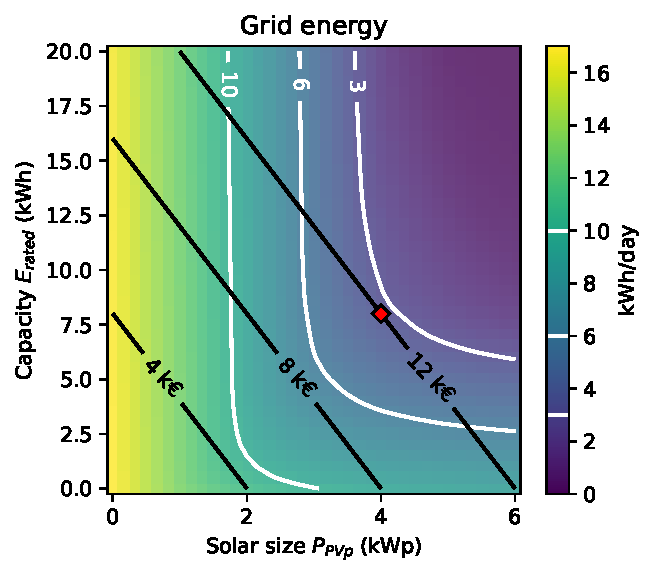
\includegraphics[width=0.8\columnwidth]{figures/Sizing_E_grid_invest_heatmap.pdf}
  \end{center}

  \caption{Effet du dimensionnement sur la consommation d'énergie réseau.
  Superposition des lignes d'iso-investissement
  }
  \label{fig:P_grid_map}
\end{figure}

La figure \ref{fig:P_grid_map} donne la puissance moyenne consommée ($\avg{P_{grid}}$)
pour chaque dimensionnement. Celle-ci est égale à 17\,kWh/j sans PV ni batterie
et baisse à mesure que $P_{PVp}$ et $E_{rated}$ augmentent\footnote{
  dans le détail,
  lorsque $E_{rated}=0$ la consommation baisse rapidement avec $P_{PVp}$
  tant qu'on ne dépasse pas 1 à 2\,kW\sub{c}. Pour intégrer davantage de PV,
  il faut ajouter une batterie.
  Inversement, pour $P_{PVp}=0$, la batterie seule ne permet pas de baisser la consommation.
  Elle pourrait néanmoins faire baisser la facture (en déplaçant la consommation)
  si une gestion optimale était employée}.
Les iso-lignes de consommation (blanches) ont une forme coudées
et nous allons montrer pourquoi c'est \emph{au niveau d'un coude que le dimensionnement est optimal}.

Nous définissons un dimensionnement optimal comme celui qui minimise le coût global sur cycle de vie,
à savoir la somme du coût d'investissement $C_{inv}$
et du coût de fonctionnement opérationnel $C_{op}$:
%
\begin{equation} \label{eq:C_tot}
  C_{tot} = C_{inv} + C_{op}
\end{equation}


Le coût d'investissement est modélisé comme proportionnel à la puissance
des panneaux et la capacité de la batterie:
%
\begin{equation} \label{eq:C_inv}
  C_{inv} = c_P P_{PVp} + c_E E_{rated}
\end{equation} 
et nous avons choisi $c_E$ = 0.5 €/kWh (source : un Tesla Powerwall de 13,5 kWh s'affiche à 7 k€)
et $c_P$ = 2 €/kW\sub{c} (optimiste pour une petite installation de 4 kW\sub{c},
mais raisonnable pour une installation ``9 à 36 kWc, ISB''\footnote{\url{http://www.photovoltaique.info/Couts-d-investissement.html}}).
Les iso-lignes d'investissement (noires) sont donc des droites inclinées
et le dimensionnement choisi coûte 12\,k€.

Le coût opérationnel $C_{op}$ est choisi égal à la facture d'électricité
sur le cycle de vie de l'installation (et donc proportionnel à la fonction-coût
du banc de test \eqref{eq:C_grid}).

\begin{equation} \label{eq:C_op}
  C_{op} = T_{life} \times \avg{c_{grid}.P_{grid} }
\end{equation} 

La durée de vie $T_{life}$ est égale à 20 ans (et exprimée en heures).
Vu que nous avons choisi une loi de gestion heuristique qui ne gère pas les heures pleines et creuses,
nous avons choisis, pour le dimensionnement uniquement, un prix de l'electricité $c_{grid}$ fixe.
Alors, le coût opérationnel \eqref{eq:C_op} est simplement proportionnel à
la consommation moyenne $P_{grid}$.
On comprend alors pourquoi, à coût d'investissement donné (cad sur une ligne noire figure \ref{fig:P_grid_map})
on a intérêt choisir le point qui tangente une courbe iso-consommation (blanche),
car il minimise le coût opérationnel. Cette tangeance est obtenu dans un coude, comme annoncé plus haut.

La position du coude dépend du niveau d'investissement choisi,
et l'on peut décrire l'ensemble des coudes comme étant environ la demi-droite
passant par les points (1\,kW\sub{c}, 0\,kWh) et (4\,kW\sub{c}, 8\,kWh).
On peut dès lors :

\begin{itemize}
 \item soit choisir a priori un investissement initial et en déduire le dimensionnement
 dans le coude correspondant.
 \item soit choisir le dimensionnement qui minimise le coût global sur cycle de vie.
\end{itemize}

\begin{figure}[!ht]
  \begin{center}
	  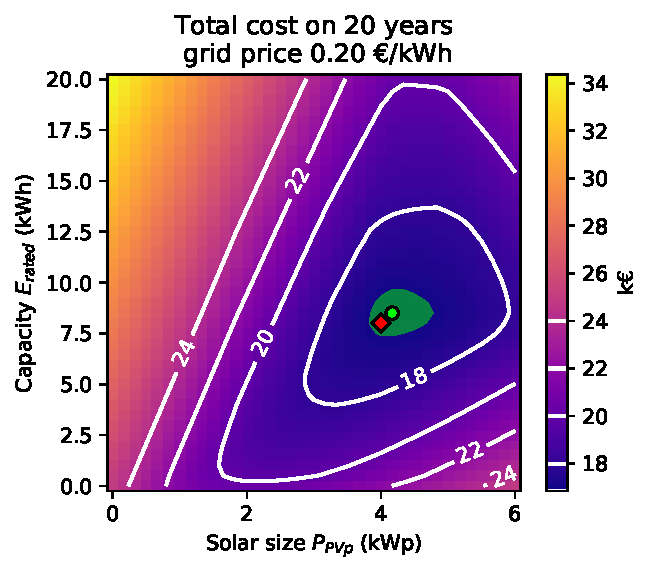
\includegraphics[width=0.8\columnwidth]{figures/Total_cost_map_grid020.pdf}
  \end{center}

  \caption{Coût total (investissement + fonctionnement)
  }
  \label{fig:cost_tot}
\end{figure}

Avec la 1\tsp{re} méthode, notre dimensionnement est l'optimum
pour un investissement de 12\,k€.
La 2\tsp{e} méthode est illustrée sur la figure \ref{fig:cost_tot},
pour un prix de l'électricité $c_{grid}$ = 0,20\,€/kWh.
Le dimensionnement que nous proposons (diamand rouge : 4\,kW\sub{c}, 8\,kWh)
est très proche de l'optimum (disque vert).
Il appartient en fait à la région quasi optimale (surlignée en vert)
où le coût total est inférieur à 101\% du minimum.
Le coût total d'environ 17\,k€ se réparti donc en 12\,k€ d'investissement
et 5\,k€ de fonctionnement (facture d'électricité sur 20 ans).

Avec la méthode qui minimise $C_{tot}$,
le résultat dépend fortement du choix de $c_{grid}$
(et de la durée d'amortissement $T_{life}$)
et nous avons donc répété l'analyse pour un prix entre 0,10 et 0,30\,€/kWh\footnote{%
  tracé animé de la figure \ref{fig:cost_tot} disponible sur le site du benchmarck}.
Il apparaît que notre dimensionnement est dans la zone quasi optimale pour un prix
entre 0,16 et 0,21\,€/kWh.


\subsection{Données de la maison solaire}
\label{ss:sol_data}

Notre banc de test est alimenté par le \emph{jeu de données réelles et ouvert} ``\href{https://www.ausgrid.com.au/Common/About-us/Corporate-information/Data-to-share/Solar-home-electricity-data.aspx}{Solar home electricity data}''
de l'opérateur Ausgrid (réseau de Sydney et sa région, Australie).
Il contient 3 années de consommation et production, au pas demi-horaire ($\Delta_t$ = 0,5\,h),
de 300 clients résidentiels disposants de panneaux PV.

Pour le banc de test, nous avons sélectionné un client sans charge pilotable\footnote{
  la description détaillée de ce choix est fournie dans le fichier \href{https://github.com/pierre-haessig/solarhome-control-bench/blob/master/data/README.md}{data/README.md} du dépôt, avec plusieurs graphiques supplémentaires.}
et nous avons choisi 30 jours consécutifs de test, du 29/11/2011 au 28/12/2011.
Les premiers jours sont représentés figure \ref{fig:testdata}
(après mise à l'échelle à 4\,kW\sub{c} de son installation PV).

\begin{figure}[!ht]
        \begin{center}
                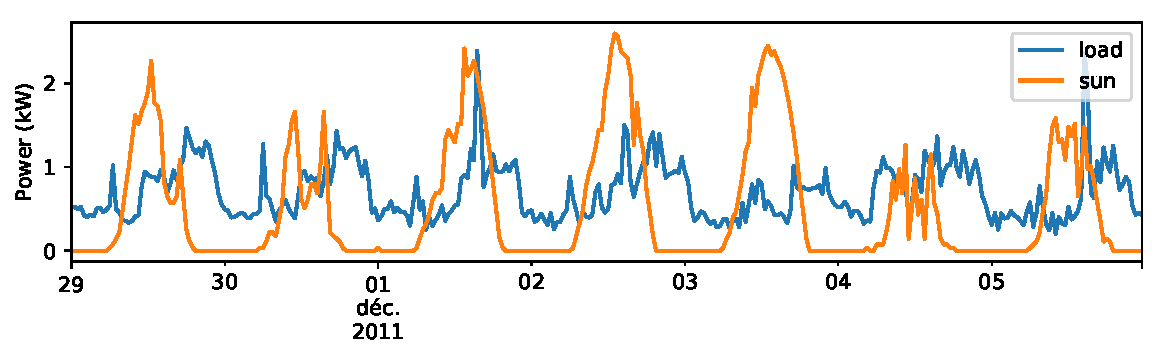
\includegraphics[width=1\columnwidth]{figures/data_week_2011-11-29.pdf}
        \end{center}

        \caption{Consommation et production PV durant les 7 jours de test
        }
        \label{fig:testdata}
\end{figure}

Les données des 30 jours précédents sont également disponibles pour une phase d'apprentissage,
par exemple pour régler la prévision d'une commande prédictive.
L'enjeu est de bien respecter la stricte séparation entre ``training set''
et ``test set'', bien connue en machine learning, et qui permet d'éviter les effets de surapprentissage
(``overfitting'').

Le tableau \ref{tab:perf_stats} donne les moyennes statistiques du productible solaire $P_{sun}$
et de la consommation souhaitée $P_{load}^*$.
Nous avons choisi d'exprimer ces moyennes en kWh/jour pour que les valeurs soient indépendantes
des la durée du test (30\,j). De plus, cela permet de mettre en regard la capacité de la batterie
(8 kWh = 1/2 journée de consommation moyenne).

% TODO: speak about bootstrap

\subsection{Accès au banc de test open source}

La description de ce modèle ainsi que les données temporelles nécessaires sont
disponibles en open source dans le dépôt GitHub \href{https://github.com/pierre-haessig/solarhome-control-bench}{pierre-haessig/solarhome-control-bench}.
Ce dépôt contient également les implémentations des méthodes de gestion d'énergie présentées dans cet article.

Il a vocation à contenir des exemples dans les langages de programmation
parmi les plus utilisés pour ce type de problème:
Matlab, Python et Julia.

\section{Approches d'optimisation}
\label{s:opt_meth}

Le but du banc de test ``maison solaire'' que nous proposons est de comparer
plusieurs lois de gestion de l'énergie pour minimiser la facture d'électricité \eqref{eq:C_tot}.
Nous présentons ici les premières stratégies que nous avons implémentées.
Le tracé temporel des 5 premiers jours du test est donné
figure \ref{fig:temporel}, pour trois méthodes différentes.

\subsection{Contrôle par règle heuristique simple}
\label{ss:heuris}

La famille de méthode gestion par des règles simples (``rule-based control'')
est la plus simple à implémenter et la plus rapide à simuler.
La limite de cette approche, c'est qu'elle repose totalement
sur ``l'inspiration'' du concepteur, c'est-à-dire sa capacité à trouver
des heuristiques pertinentes.

Pour le cas de la maison solaire, si l'on s'en tient à minimiser
la consommation d'énergie (moyenne de $P_{grid}$),
par opposition à la facture (moyenne de $c_{grid}.P_{grid}$),
voici une stratégie très efficace:
%
\begin{equation} \label{eq:heuris_sto}
  P_{sto} = -P_{nl} = P_{sun} - P_{load}^*, \text{ tant que possible}
\end{equation}
%
où tant que possible signifie que la batterie n'est pas pleine ou vide,
selon le signe de $P_{nl}$.
On utilise les variables auxiliaires définies parties \ref{sss:auxi_var}.
Si l'équation \eqref{eq:heuris_sto} est applicable, alors on déduit
de la conservation de la puissance \eqref{eq:cons2} que $P_{gc} = 0$,
c'est-à-dire $P_{grid} = 0$ (on ne consomme rien) et
$P_{curt} = 0$ (on ne gâche pas de productible solaire).
C'est bien une heuristique prometteuse car cette décision est gratuite
sur l'instant.

Inversement, si \eqref{eq:heuris_sto} est inapplicable,
c'est que la batterie est saturée donc $P_{sto} = 0$
et la variable $P_{gc}$ sert de recours,
toujours pour assurer la conservation de la puissance \eqref{eq:cons2}:
%
\begin{equation}
  P_{gc} = P_{grid} - P_{curt} = P_{nl} = P_{load}^* - P_{sun}
\end{equation}

Comme $P_{grid}$ et $P_{curt}$ sont exclusives, deux sous-cas se présentent:
\begin{itemize}
 \item si $P_{nl}>0$ (c.-à-d. consommation > productible et batterie vide),
 le réseau prend le relais: $P_{grid} = P_{nl}$
 \item si $P_{nl}<0$ (c.-à-d. productible > consommation et batterie pleine),
 il faut écrêter la production: $P_{curt} = - P_{nl}$
 (ou autrement dit, $P_{pv}$ est ajustée égal à $P_{load}^*$)
\end{itemize}

Ce comportement est visible sur en haut de la figure \ref{fig:temporel},
où l'on observe que pendant une grande partie du temps,
la batterie suit la charge nette (charge si production, décharge si forte consommation)
et le recours $P_{gc}$ est constant égal à zéro.
Si la batterie est vide, et tant que la consommation domine,
le réseau prend le relais ($P_{gc}>0$, souligné en rouge)
Inversement si la batterie est pleine, et tant que la production solaire domine,
l'écrêtage intervient ($P_{gc}<0$, souligné en jaune).

L'analyse quantitative des résultats (tableau \ref{tab:perf_stats}, ligne ``heuristique'')
montrent que la consommation d'énergie ($\avg{P_{grid}}$ = 3,38\,kWh/j) est minimale, car égale à celle de 
l'optimisation anticipative qui minimise la consommation, ligne ``optim. éner.'').
Par contre, la facture n'est pas optimale, car cette méthode ne tient pas compte
des heures creuses. D'ailleurs, on observe figure \ref{fig:temporel}
que l'appel au réseau ($P_{gc}>0$) ne se fait pas préférentiellement pendant
les périodes bleu clair.

La limite de cette méthode de gestion d'énergie est donc le pendant négatif
de sa simplicité : il est difficile d'intégrer des complexités du problème
tel que des tarifs flexibles.

\subsection{Programmation dynamique}
La programmation dynamique\cite{Bertsekas:2005:DPOC_vol1} est un
excellent cadre théorique pour poser un problème de gestion avec entrées incertaines (stochastique).
Point particulier, elle nécessite une modélisation des incertitudes par un \emph{processus markovien}\cite{Haessig:2013:ESPy}.
L'implémentation numérique est impossible
si la dimension de l'état est trop grande (>4).

Pour la maison solaire, qui n'a qu'une batterie (1 variable d'état),
la programmation dynamique devrait être utilisable.
Pour l'instant, la modélisation markovienne de l'entrée incertaine ($P_{nl}$) reste à faire.
Une des difficultés est la prise en compte du caractère non stationnaire
du processus, car production et consommation dépendent fortement de l'heure du jour.
La variable $hod$ doit donc être ajoutée à l'état.
La prise en compte de l'autocorrélation de l'entrée se fait également par augmentation
de l'état\cite[§1.4]{Bertsekas:2005:DPOC_vol1}.
Pour garder la dimension de l'état $\leq 3$, on n'a le droit qu'à un processus d'ordre
au plus 1 pour modéliser l'autocorrélation.
Le travail de modélisation est donc très contraint.

Une fois ce travail de modélisation effectué, l'objectif sera d'obtenir une loi de gestion
à l'aide du package Python \texttt{stodynprog}\cite{Haessig:2013:ESPy}.


\begin{table}
%% increase table row spacing, adjust to taste
\renewcommand{\arraystretch}{1.2}

\caption{Performance des différentes méthodes de gestion d'énergie}
\label{tab:perf_stats}

\noindent
\centering
  \begin{minipage}{\linewidth} %Use the minipage environment to footnote tables
  \renewcommand\footnoterule{\vspace*{-5pt}} %to remove the horizontal rule above the table footnote
  \begin{center}
    \begin{tabular}{c c c c c}
      \toprule
      \multirow{2}{*}{Méthode} & \multicolumn{4}{c}{Moyennes journalières (kWh/j, \texteuro/j)} \\
      \cline{2-5}
	& $P_{sto}$
        & $P_{curt}$
        & $P_{grid}$
        & $c_{grid}.P_{grid}$
        \\
      \midrule
      heuristique
          & 0.03
          & 1.94
          & 3.38
          & 0.563\\
      MPC
          & 0.03
          & 2.94
          & 4.38
          & 0.543\\
      MPC anticip.
          & 0.03
          & 1.94
          & 3.38
          & 0.354\\
      optim. anticip.
          & 0.00
          & 1.97
          & 3.38
          & 0.354\\
      optim. éner.
          & 0.00
          & 1.97
          & 3.38
          & 0.631\\
      \bottomrule
    \end{tabular}
  \end{center}
  \end{minipage}
\end{table}

\begin{figure}
  \begin{center}
    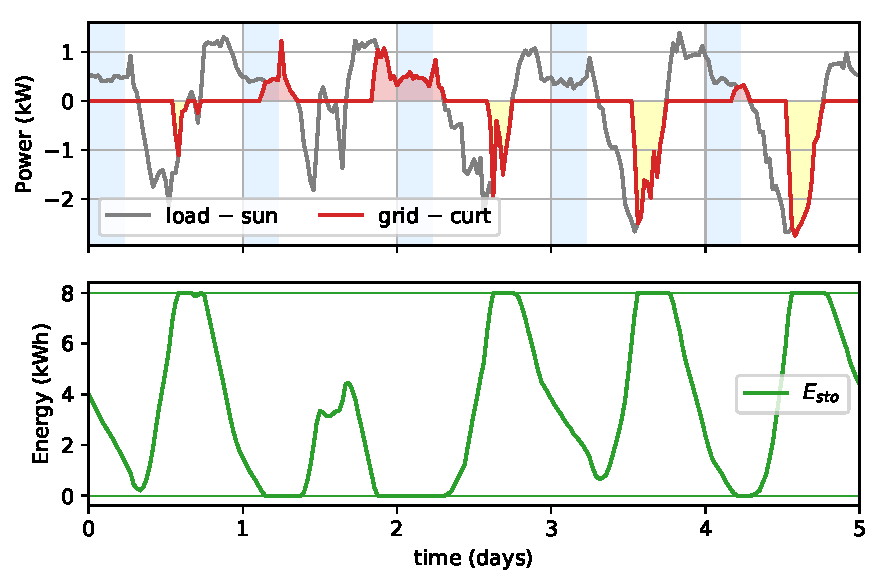
\includegraphics[width=1\columnwidth]{figures/matlab_rule-based.pdf}
    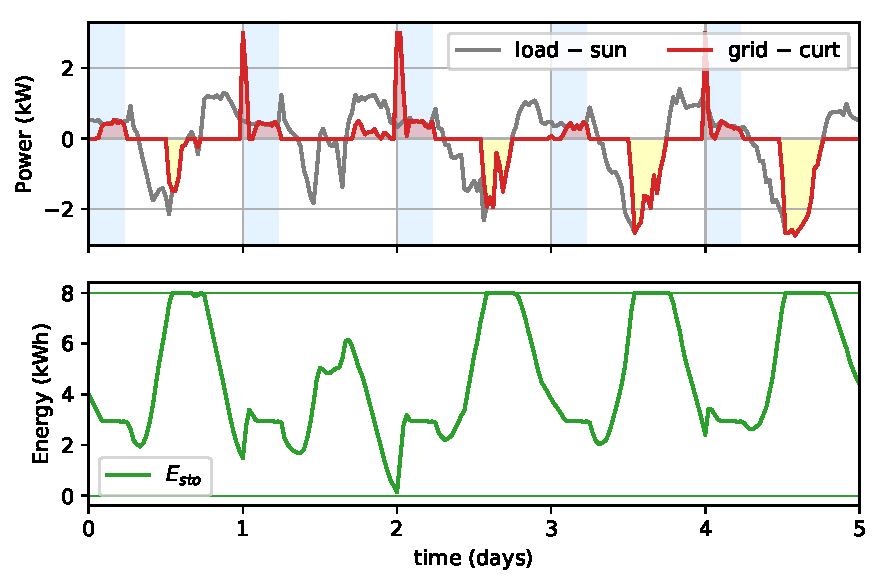
\includegraphics[width=1\columnwidth]{figures/matlab_mpc.pdf}
    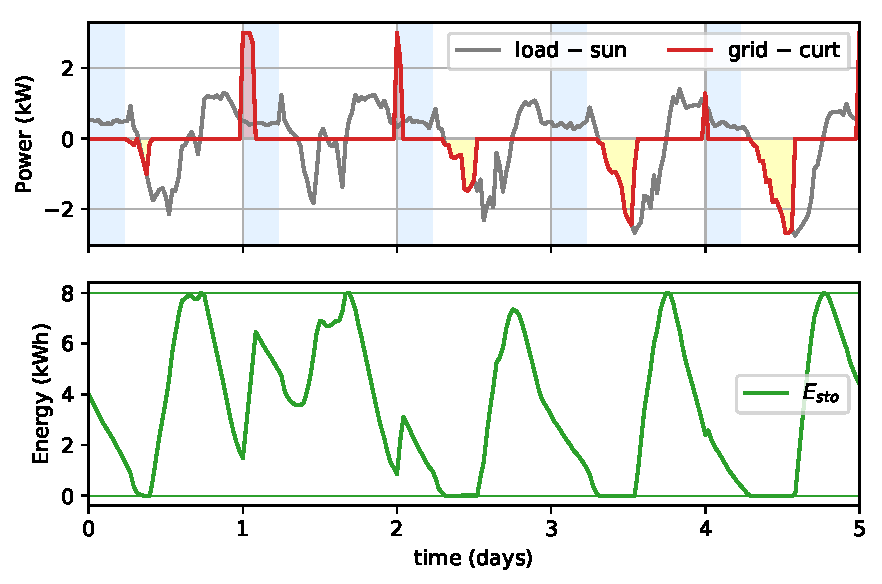
\includegraphics[width=1\columnwidth]{figures/julia_anticipative.pdf}
  \end{center}

  \caption{Tracé temporel des 5 premiers jours du test pour trois méthodes
  de gestion d'énergie de la maison solaire.
  Donnée d'entrée $P_{nl}$ en gris, décisions $P_{gc}$ en rouge (§\ref{sss:auxi_var})
  et énergie stockée $E_{sto}$ en vert.
  L'appel au réseau ($P_{gc}>0$) est rempli en rouge clair,
  alors que l'écrêtage ($P_{gc}<0$) est rempli en jaune clair.
  Les périodes bleu clair marquent les heures creuses.
  De haut en bas (du moins performant au plus performant):
  règle heuristique simple (§\ref{ss:heuris}),
  commande prédictive (MPC) avec prévision non anticipative (§\ref{ss:mpc}),
  optimisation déterministe anticipative (§\ref{ss:anticip}).
  Pour l'optimisation anticipative, la performance est artificiellement bonne,
  car la décision d'un instant dépend de données futures.
  }
  \label{fig:temporel}
\end{figure}

\subsection{Optimisation déterministe anticipative}
\label{ss:anticip}

Cette méthode consiste en une optimisation globale de la trajectoire des signaux
sur tout l'horizon du problème (30 jours pour notre test), en utilisant
la valeur des données d'entrées.
Toutefois, cela implique que la décision sur les premiers instants dépend
de données futures! La performance est donc articiellement bonne (coût sous-évalué),
car ces données ne sont pas connus en pratique.
Cette méthode n'est donc pas implémentable in situ.
Une variante plus réaliste et très courante est la commande prédictive
(cf. partie suivante \ref{ss:mpc}), à condition de ne pas l'utiliser
avec une prévision anticipative. La simulation est par contre plus coûteuse,
car une optimisation doit être effectuée à chaque pas de temps.

L'optimisation anticipative est utilisée dans plusieurs études scientifiques,
en particulier de dimensionnement (\cite{Rigo-Mariani:2014:SGE}),
car elle fournie une ``baseline de performance''
plus attrayante qu'une gestion empirique.
Cependant, nous pensons que cette approche est risquée, car il n'y a aucune maitrise
du niveau de sous-évaluation du coût par rapport à une gestion réel.

Sur la maison solaire, vu le modèle présenté partie \ref{ss:model},
la fonction coût est linéaire en la variable de décision $P_{grid}$
et des contraintes sont linéaires aussi.
Le problème d'optimisation est donc du type ``programme linéaire''
qui est très efficacement soluble malgré la taille
($30 \times 48 = 1440$ pas de temps, avec plusieurs variables de décision).
Nous l'avons implémenté en Julia avec le package JuMP\cite{Dunning:2017:JuMP}
(outil de modélisation comparable à AMPL ou GAMS, mais implémenté en Julia
et open source).

Nous avons implémenté deux variantes du problème
et les résultats quantitatifs sont présentés dans le tableau \ref{tab:perf_stats}:
%
\begin{itemize}
  \item optimisation de la facture (ligne ``optim. anticip.'')
  \item optimisation de la consommation énergétique (ligne ``optim. éner.''),
  équivalente à une minimisation de la facture, mais avec un prix fixe
\end{itemize}

Nous déduisons trois faits des résultats d'optimisation:
\begin{itemize}
 \item le minimum ``absolu'' de la facture (connaissant parfaitement le futur)
 est de 0,354\,€/kWh, nettement mieux qu'une gestion heuristique.
 \item les deux objectifs d'optimisation donnent la même consommation d'énergie
 (3.38\,kWh),
 c'est-à-dire que la minimisation de la facture se fait par déplacement
 de bloc d'énergie à l'échelle d'une journée, sans consommer plus.
 \item la gestion heuristiques obtient la même consommation,
 donc la connaissance du futur n'apporte aucun gain énergétique,
 seulement un gain financier.
\end{itemize}

Sur le bas de la figure \ref{fig:temporel}, on peut analyser qualitativement
la gestion d'énergie. En particulier, on observe que la recharge de la batterie
par appel au réseau se fait presque exclusivement la nuit.
Par ailleurs, la quantité d'énergie appelée dépend nettement de la production solaire
\emph{de la journée suivante} (grosse recharge nocturne sur faible production future,
pas de recharge nocture si forte production future).
L'effet d'anticipation joue donc bien un rôle important.

\subsection{Commande prédictive (MPC)}
\label{ss:mpc}

La commande prédictive (MPC) utilise une \emph{prévision ponctuelle (moyenne)} des entrées incertaines.
Elle compense l'erreur de prévision en répétant l'optimisation sur un \emph{horizon glissant}.
L'implémentation numérique est efficace si le problème d'optimisation est linéaire (ou en tout cas convexe),
ce qui est le cas ici.

Des variantes du MPC déterministe existent pour mieux faire face à l'incertain: le MPC stochastique,
qui utilise un \emph{ensemble de scénarios}, éventuellement avec un ``recours affine''.

\begin{figure}[!ht]
        \begin{center}
                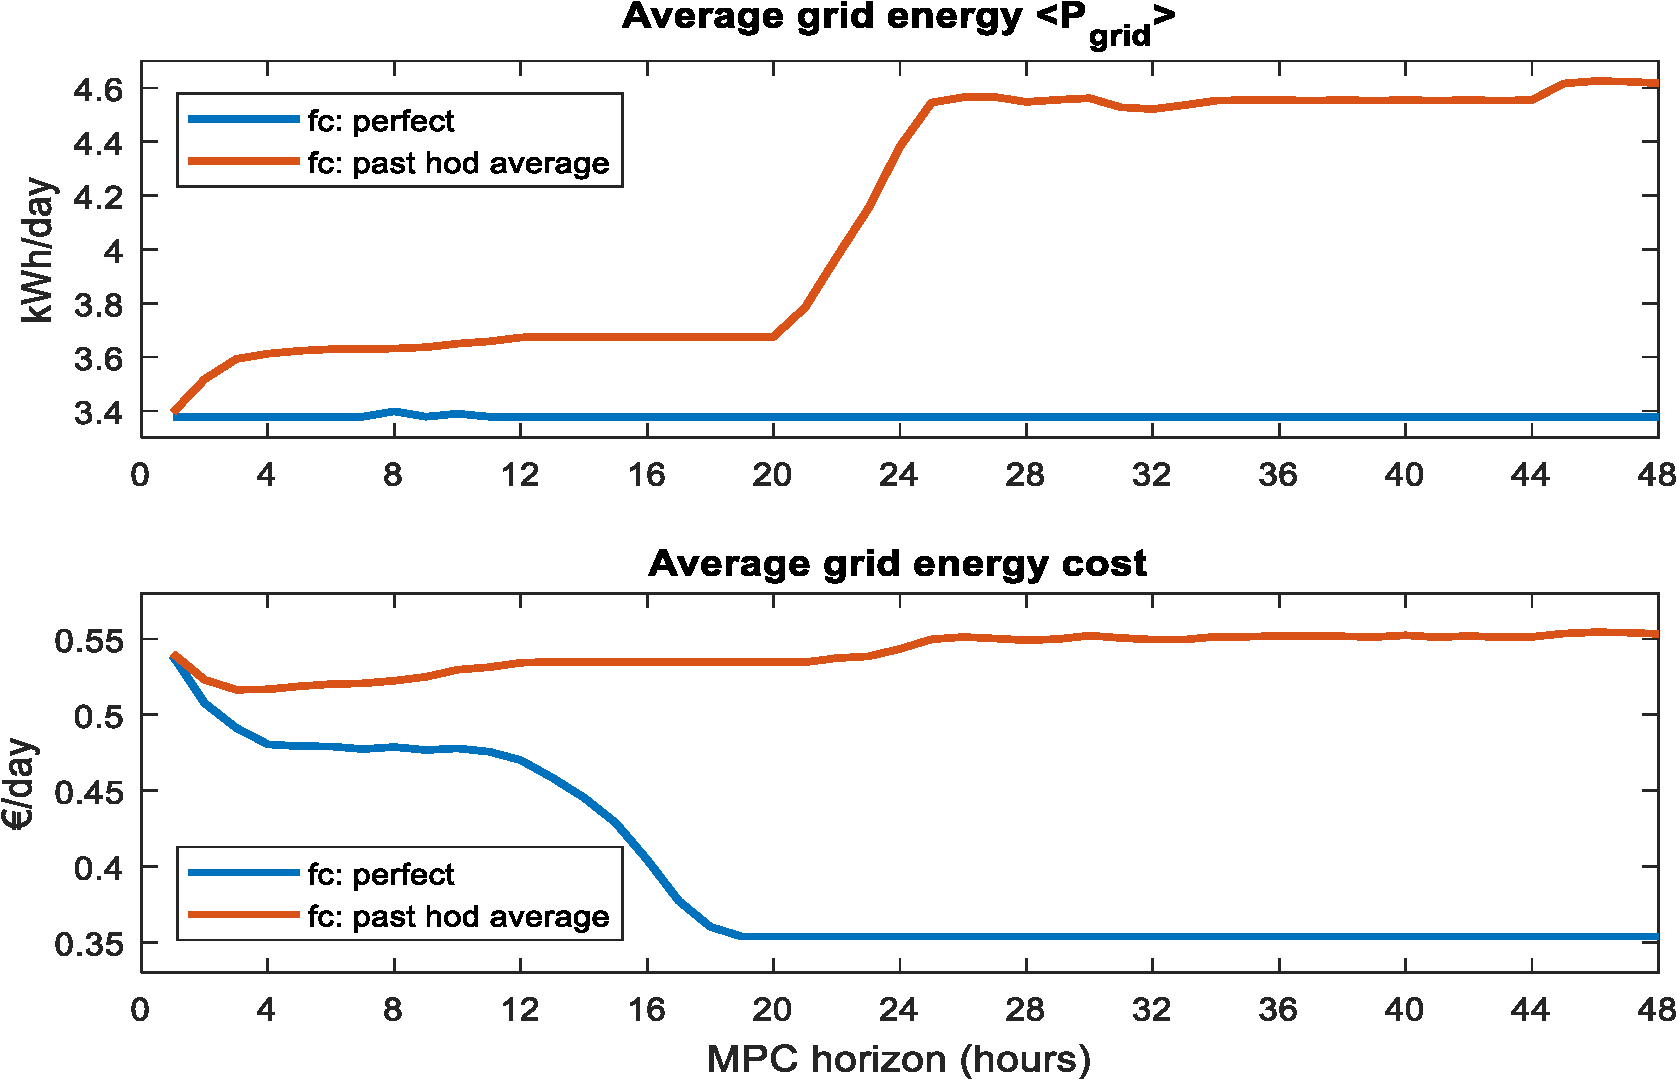
\includegraphics[width=1\columnwidth]{figures/MPC_horizon_effect.pdf}
        \end{center}

        \caption{Effet de l'horizon du contrôle MPC sur la performance (consommation d'énergie en haut, coût de cette énergie en bas).
        Courbes bleues: MPC alimenté par une prévision parfaite (anticipative) du futur.
        Courbes rouges: MPC alimenté par une prévision non anticipative, égale à la moyenne passée à chaque heure du jour. 
        }
        \label{fig:mpc_horiz}
\end{figure}

%\subsection{MPC stochastique et robuste}

%une amélioration du MPC déterministe.

% \subsection{Commande prédictive non-linéaire}
% 
% Optimica JModelica.org \cite{Akesson:2010:CCE}
% 
% sareni sge 2014 \cite{Rigo-Mariani:2014:SGE} : optim linéaire puis reprojection.

\subsection{Comparaison}




\section{Conclusions}

Le banc de test pour la gestion d'énergie d'une maison solaire
doit permettre de faciliter l'accès à une palette de méthode de gestion
sur un exemple simple mais réaliste (e.g. données de production solaire et de consommation réelles).

Perspectives : ce banc de test pour la gestion d'énergie,
à dimensionnement fixé, est une première étape pour l'étude des méthodes
de dimensionnement optimal qui prennent en compte l'optimisation de la loi de gestion
\cite{Haessig:2014:SGE}.

% structure de décision dans un contexte multi-agent (pas abordé ici
% car focus sur optimisation d'un système individuel) : centralisé, distribué,
% mécanisme de prix, multi-agent...

\bibliographystyle{IEEEtran}
\bibliography{00_References}

\end{document}